\chapter{Análisis de resultados} \label{cap:analisideresultado}

En este capitulo se analizan los distintos resultados obtenidos en nuestros experimentos, detallados en la \autoref{cap:experimentos}, se comparan con los de Bansal \etal~\cite{bansal2018zero} y se explican las diferencias obtenidas.

\section{Resultados cuantitativos} \label{sec:resultadoscuantitativos}

Esta sección desarrolla de forma numérica los resultados obtenidos por los distintos modelos y en las distintas métricas. Se analizan las configuraciones ZSD Y GZSD.

\subsection{Resultados ZSD}

\begin{table}[H]
	\centering
	\resizebox{12.5cm}{1cm} {
		\begin{tabular}{|l|c|c|c|c|c|}
			\hline
			\multicolumn{1}{|c|}{\textbf{Métrica}} & \textbf{Baseline \cite{bansal2018zero}} & \multicolumn{1}{l|}{\textbf{DSES \cite{bansal2018zero}}} & \textbf{Nuestros con VGG} & \textbf{Nuestros con ResNet} & \multicolumn{1}{l|}{\textbf{Mejor  resultado de \cite{rahman2020zero}}} \\ \hline
			\textbf{100@Recall (Bansal)}           & 22.14                                   & 27.19                                                    & 26.34                     & 28.91                        & -                                                                       \\ \hline
			\textbf{100@Recall}                    & -                                       & -                                                        & 5.44                      & 6.38                         & 12.27                                                                   \\ \hline
			\textbf{mAP@0.5}                       & 0.32                                    & 0.54                                                     & 0.19                      & 0.23                         & 5.05                                                                    \\ \hline
			\textbf{mAP@[.5, .95]}                 & -                                       & -                                                        & 0.17                      & 0.21                         & -                                                                       \\ \hline
		\end{tabular}
	}
	\caption{Resultados obtenidos por Bansal \etal~\cite{bansal2018zero}, nosotros y Rahman \etal~\cite{rahman2020zero}. Se presentan las distintas métricas \textit{recall} y \textit{mAP}, evaluados en COCO.}
	\label{tab:resultadosZSD}
\end{table}

La idea inicial de esta tesis era replicar el modelo base de Bansal \etal~\cite{bansal2018zero}, una ves logrado esto, modificar nuestra implementación con el objetivo de mejorar los resultados. Pero esta idea se frustro al no obtener valores similares a los reportados. Para encontrar la causa de esta diferencia se necesito depurar cada etapa del código. Luego de confirmar que la implementación no tenia ningún error aparente y replicaba correctamente lo que se define en el trabajo de Bansal \etal~\cite{bansal2018zero}, se comenzó a modificar los distintos parámetros de cada etapa, aun sin éxito, se analizaron las métricas, y como ya se explico anteriormente se encontró una diferencia en la definición, esto explica la discrepancia en los resultados que analizaremos a continuación.  

La \autoref{tab:resultadosZSD}, muestra los valores de las métricas \textit{100@Recall}, en la versión desarrollada por Bansal \etal~\cite{bansal2018zero} y la de Padilla \etal~\cite{padilla2020survey}, también se muestran los resultados para \textit{mAP@0.5} y \textit{mAP[.5, .95]}. Se observan 2 modelos propuestos por nosotros, uno utilizando \textit{VGG16} y el otro \textit{Inception ResNet V2}, ademas se agregan los mejores resultado presentado por el trabajo de Rahman \etal~\cite{rahman2020zero}. Se eligió este documento ya que es un trabajo más actual y aborda de una manera similar a la nuestra el problema de ZSD, aunque presenta algunas mejoras y un modelo más complejo.\\

La \textit{100@Recall} es un buen punto de partida para analizar el modelo propuesto, ya que refleja el numero de propuestas predichas correctamente sobre el total de cuadros verdaderos. Obtuvimos 6.38 puntos en esta métrica, que resulta por debajo de lo esperado. Pero esto no significa necesariamente que el modelo no funciona correctamente, existen varios parámetros que influyen en este resultado. El punto que más afecta es el generador de propuestas, ya que menos del 50\% de los cuadros verdaderos obtienen una propuesta con $IoU > 0.5$ lo cual reduce mucho la esperanza de esta métrica. Otro punto, es la capacidad de la CNN de obtener un espacio de características visuales, que agrupe las clases visualmente similares y separe las diferentes. Como se vio en la \autoref{ssec:experimentacionconcnn}, \textit{ResNet} supera a \textit{VGG16} en esta tarea, lo cual se refleja en la pequeña mejora del modelo que utiliza  \textit{ResNet}.

En cuanto a \textit{mAP} obtuvimos 0.23 puntos, esto es un bajo desempeño comparado con los trabajos publicados por la comunidad científica. Pero al igual que \textit{100@Recall} se ve afectada por los puntos antes mencionados, ademas, existe otro que la afecta muy fuertemente. Por la naturaleza de la matriz que proyecta las caracteristicas visuales al espacio semantico, hace que dos objetos proyectados obtengan una similitud coseno poco distanciada, la cual ronda entre los valores 0.3 y 0.6. Es decir que si proyecto dos imágenes con muy pocas diferencias obtendrán un similitud como máximo de 0.6. Esta similitud es utilizada como el puntaje de confianza de una predicción y como se explico en la \autoref{ssec:definiciondemetricas}, \textit{mAP} varia un limite de confianza de predicciones para calcular la curva AUC. Esto hace que para limites superiores a 0.6 se obtengan valores muy bajos o incluso nulos de \textit{precisión}.\\
 

En comparacion con el mejor resultado de Bansal \etal~\cite{bansal2018zero} el cual denomina \textit{Densely Sampled Embedding Space (DSES)} y consiste en aumentar el procedimiento de entrenamiento con datos adicionales de fuentes externas que contienen casillas que pertenecen a clases distintas a las clases invisibles. Obtiene 27.19 puntos en su definición de \textit{recall}, el cual nuestro modelo base supera con 28.91 puntos usando \textit{ResNet}. Esto se debe a que en la etapa de depuración se modificaron algunos parapetaros por defecto del entrenamiento, como el numero de lote, la taza de aprendizaje, el optimizador, etc.  

En cuanto mAP, Bansal no aporta mucha información y su implementación es desconocida, por lo cual asumimos que lo reportado es \textit{mAP@0.5}. De inmediato se puede observar que los valores son muy bajos 0.54. Esto genera una discrepancia con su alto rendimiento de \textit{recall} y refleja lo poco representativa de esta ultima métrica. 

Si comparamos con un trabajo más actual~\cite{rahman2020zero} que obtiene 12.27 en \textit{100@Recall} y un excelente desempeño en \textit{mAP@0.5} con 5.05 puntos, refleja una consistencia con nuestros valores y que la implementación utilizada para calcular las métricas esta mejor encaminada.\\
	

Estos resultados fueron calculados sobre la división de clases propuesta por Bansal ya que ambos trabajos con cuales comparamos utilizan esta. Pero también se corrieron las evaluaciones con la partición propuesta en este trabajo. Los resultados se vieron afectados entre un 4\% y 7\% menos al utilizar nuestra división. Esta reducción se debe a que el documento de Bansal \etal~\cite{bansal2018zero} utiliza como criterio de división los vectores semánticos de las clases, esto afecta positivamente ya que es el mismo espacio utilizado para inferir las clases invisibles.\\

También se calcularon las métricas para el conjunto de datos CIFAR-ZSD. Pero fueron necesario algunas mejoras para adaptarse a las diferencias con COCO. Primero se utilizo una tamaño de la entrada de la CNN más pequeña de 32x32. Esto se debe a que las imágenes no tienen una gran resolución. También, se reduzco considerablemente el numero máximo de de propuestas, del orden de 50. La justificación de esto es que los objetos sobresalen del fondo de la imagen y es más fácil su detección.

Dicho esto, los resultados obtenidos fueron, 8.83 en \textit{100@Recall} (implementación de Padilla \etal~\cite{padilla2020survey}) y 0.72 para \textit{mAP@0.5}. Estos valores al contrario de los reportados para COCO, se ven influenciado por la calidad de la imagen, lo que hace muy difícil de diferenciar el aspecto visual de las distintas clases.\\

En conclusión, sabiendo que es solo un modelo base muy sencillo sin utilizar ningún tipo de información extra, obtuvimos valores aceptables para \textit{100@Recall}, aunque resulta importante resaltar su bajo desempeño en \textit{mAP}. 

\subsection{Resultados GZSD}
Por ultimo, se analizaron los resultados en el desafió de GZSD. La configuración generalizada de aprendizaje sin ejemplos es más realista que la configuración de aprendizaje sin ejemplos discutida anteriormente, porque tanto las clases visibles como las invisibles están presentes durante la evaluación.

La \autoref{tab:resultados-gzsd}, se muestra los resultados para GZSD evaluados en COCO. En esta se puede observar el desempeño obtenido en \textit{100@Recall} y \textit{mAP@0.5}, para las cuales este trabajo obtuvo 3.84 puntos y 0.13 respectivamente en promedio con las clases visibles e invisibles. Como es de esperarse se obtuvo un mejor rendimiento para las clases vistas en ambas métricas.

La metodología de evaluacion es la misma que ZSD estándar solo que ahora se agrega las clases visibles a las pruebas. Algunos trabajos modifican la metodología de evaluacion para que las clases invisibles tengan más oportunidad sobre las vistas, pero esto agrega información extra que en situaciones reales no tenemos.\\

Si comparamos los resultados de ZSD vs GZSD, se observa un decremento en los valores de las métricas promedio. Esta disminución también se ve reflejado en los trabajos \cite{bansal2018zero} y \cite{rahman2020zero}. El motivo de esto es que las clases vistas al estar en entrenamiento, tienden a tener un mejor puntaje en la etapa de evaluacion que las clases invisibles perteneciente a su clase superior. Por esto muchos objetos que en la configuración anterior, predecía correctamente ahora una clase visible obtiene mejor puntaje.\\


\begin{table}[]
	\centering
	\resizebox{12.5cm}{1.2cm} {
	\begin{tabular}{|l|c|c|c|}
		\hline
		\multicolumn{1}{|c|}{\multirow{3}{*}{Modelo}} & \multicolumn{3}{c|}{GZSD}                                                       \\ \cline{2-4} 
		\multicolumn{1}{|c|}{}                        & Clases vistas             & Clases Invisibles        & Media                    \\ \cline{2-4} 
		\multicolumn{1}{|c|}{}                        & mAP/Recall Bansal/Recall  & mAP/Recall Bansal/Recall & mAP/Recall Bansal/Recall \\ \hline
		Mejor resultado \cite{bansal2018zero}                                        & -/15.02/-                 & -/15.32/-                & -/15.17/-                \\ \hline
		Nuestro modelo base                              & 0.15/20.98/4.77           & 0.11/18.53/2.92          & 0.13/19.75/3.84           \\ \hline
		Mejor resultado de \cite{rahman2020zero}     & 13.93/-/20.42             & 2.55/-/12.42             & 4.31/-/15.45             \\ \hline
	\end{tabular}
	}
	\caption{Resultados obtenidos, en el desafió GZSD, para los modelos de Bansal \etal~\cite{bansal2018zero}, nuestro (ResNet) y Rahman \etal~\cite{rahman2020zero}}
	\label{tab:resultados-gzsd}
\end{table}
\newpage

\section{Resultados cualitativos} \label{sec:resultadoscualitativos}

Para poder tener una idea más realista del comportamiento del modelo propuesto, se probo sobre algunas imágenes de muestra. Con el objetivo de obtener ejemplos más claro fue necesario modificar la metodología que se utilizo para calcular los resultados cuantitativos. Para esto, disminuimos el numero de propuestas en el orden de 10 y se descarto todas aquellas que obtuvieron un puntaje de confianza menor a 0.5. Esto hace que los ejemplos solo contengan los objetos más relevantes, pero una contra de esto es que descarta muchos que están en un segundo plano. Otra aclaración importante es que se evaluá ZSD y no GZSD, es por esto que se ignoran o confunde clases visibles. 

La \autoref{fig:ejmeplosModelo} muestra las detecciones del modelo propuesto en el conjunto de datos COCO. Los cuadros azules muestran detecciones incorrectas y en verdes los que acertaron a la clase que pertenece el objeto. 

Si bien el modelo confunde algunas instancias de objetos, cabe destacar que por lo general se equivoca dentro de una misma clase superior, confirmado que el modelo propuesto es capaz de relacionar aspectos visuales y detectar clases invisibles sin observar ninguna muestra durante el entrenamiento. 

Otro punto es que a pesar de que reducimos la cantidad de propuestas, no están centradas en los objetos y no detectan otros que se encuentran en un primer plano. Ademas con esta configuración resulta difícil encontrar un ejemplo que se observen objetos pequeños como  un ``cuchillo'' ya que las propuestas son a escalas más grandes y se ven opacadas por los objetos que lo rodean como un ``plato''.

\begin{figure}[]
	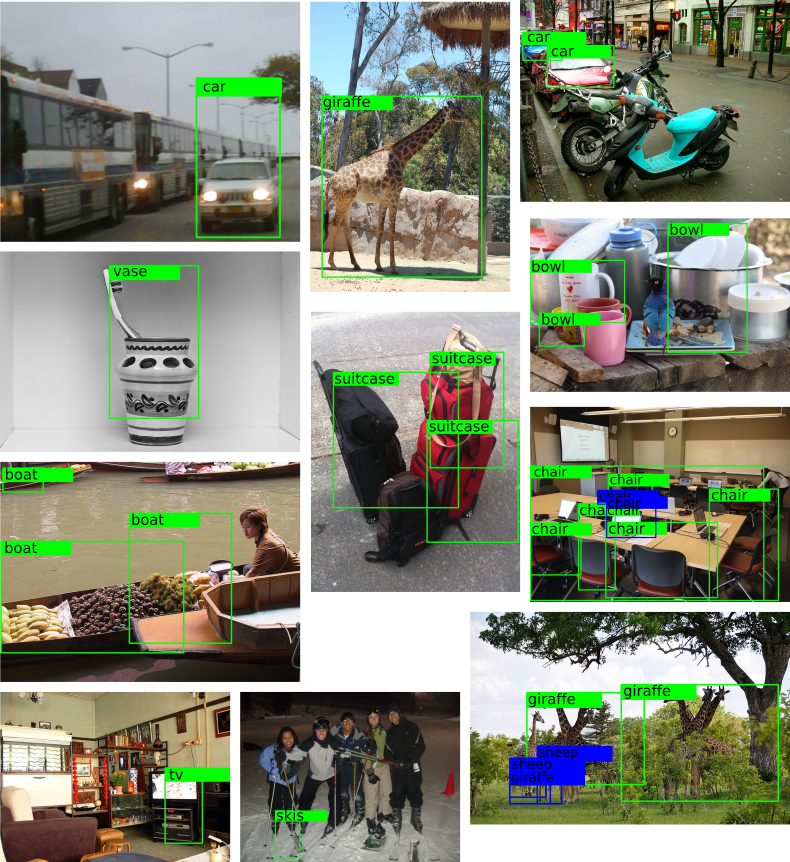
\includegraphics[width=1\textwidth]{dibujo.png}
	\caption{Ejemplo del comportamiento del modelo sobre clases invisibles. Los cuadros azul son las predicciones incorrectas y en verde las correctas.}
	\label{fig:ejmeplosModelo}
\end{figure}
